\chapter{Détection d'Anomalies par Machine Learning}

\section{Pipeline de traitement des données}

\subsection{Chargement et exploration}

Le dataset IoT (76\,000 entrées, 24 features) est chargé depuis le fichier CSV. Une exploration descriptive préalable a permis d'identifier les caractéristiques statistiques de chaque classe.

\begin{figure}[H]
  \centering
  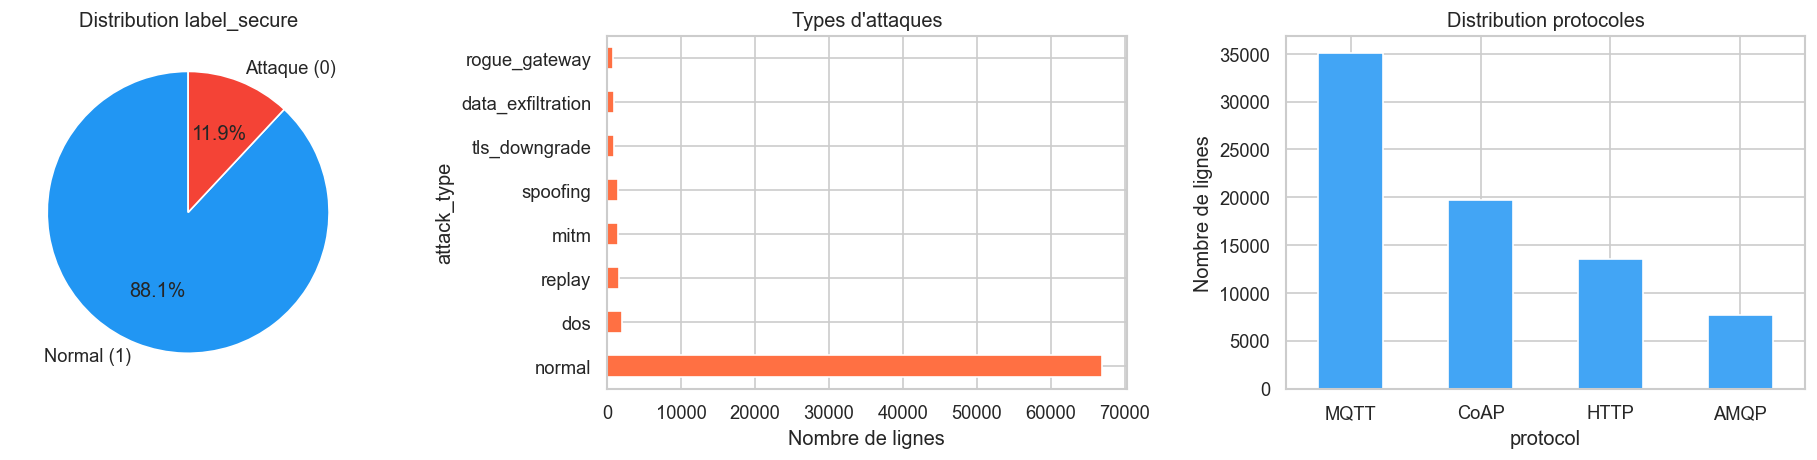
\includegraphics[width=0.8\textwidth]{figures/eda_classes_distribution.png}
  \caption{Distribution des classes dans le dataset (EDA)}
  \label{fig:eda_classes}
\end{figure}

\begin{figure}[H]
  \centering
  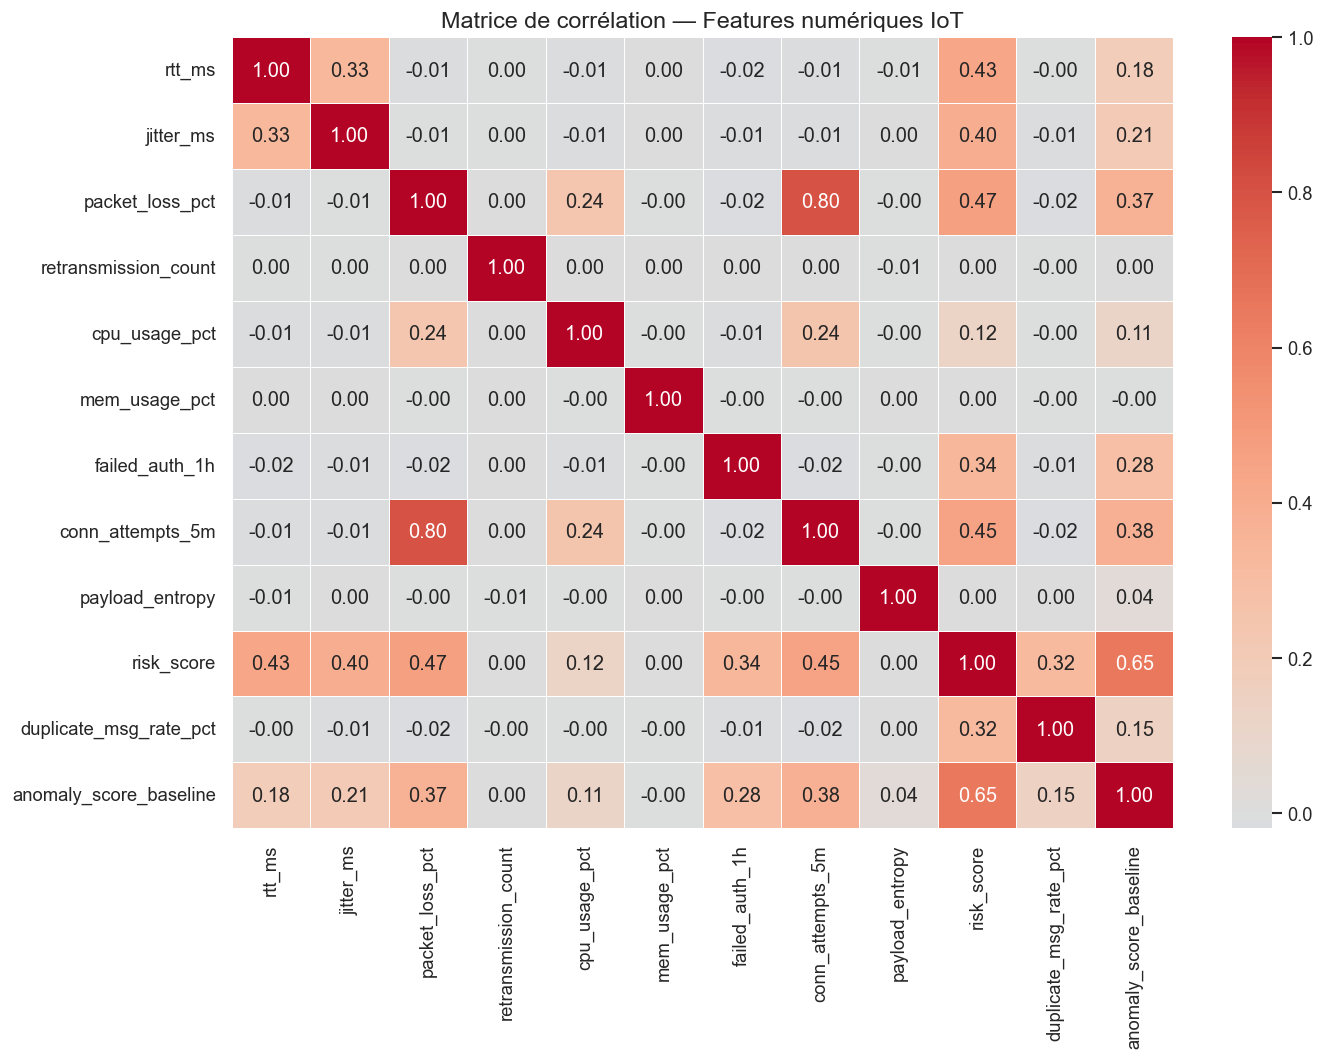
\includegraphics[width=\textwidth]{figures/eda_correlation_heatmap.png}
  \caption{Matrice de corrélation des features}
  \label{fig:eda_corr}
\end{figure}

\subsection{Prétraitement}

\begin{lstlisting}[language=python, caption=Pipeline de prétraitement des données IoT]
from sklearn.preprocessing import LabelEncoder, StandardScaler
from sklearn.model_selection import train_test_split

# Encodage des variables catégorielles
le = LabelEncoder()
df['attack_encoded'] = le.fit_transform(df['attack_type'])
df['binary_label'] = (df['attack_type'] != 'Normal').astype(int)

# Sélection des features (suppression identifiants, timestamps)
feature_cols = [c for c in df.columns if c not in 
                ['attack_type', 'attack_encoded', 'binary_label',
                 'timestamp', 'flow_id']]

X = df[feature_cols]
y_binary = df['binary_label']
y_multi = df['attack_encoded']

# Normalisation
scaler = StandardScaler()
X_scaled = scaler.fit_transform(X)

# Split train/test stratifié
X_train, X_test, y_train, y_test = train_test_split(
    X_scaled, y_binary,
    test_size=0.2, random_state=42, stratify=y_binary
)
\end{lstlisting}

\section{Isolation Forest — Détection non supervisée}

\subsection{Principe et configuration}

L'IsolationForest isole les anomalies en construisant des arbres binaires aléatoires. Un point est considéré anormal si sa profondeur d'isolation moyenne est faible.

\begin{lstlisting}[language=python, caption=Entraînement de l'IsolationForest]
from sklearn.ensemble import IsolationForest

iso_forest = IsolationForest(
    n_estimators=200,
    contamination=0.43,   # proportion d'anomalies estimée
    max_features=1.0,
    random_state=42,
    n_jobs=-1
)

# Entraînement sur données non-étiquetées (X seulement)
iso_forest.fit(X_train)

# Prédiction : -1 = anomalie, 1 = normal
y_pred_iso = iso_forest.predict(X_test)
y_pred_iso_binary = (y_pred_iso == -1).astype(int)
\end{lstlisting}

\subsection{Résultats IsolationForest}

\begin{table}[H]
\centering
\caption{Métriques IsolationForest (détection binaire normale/anomalie)}
\label{tab:iso_results}
\begin{tabular}{ll}
\toprule
\textbf{Métrique} & \textbf{Valeur} \\
\midrule
Précision & 0.927 \\
Rappel & 0.933 \\
F1-Score & \textbf{0.930} \\
ROC-AUC & \textbf{0.959} \\
\bottomrule
\end{tabular}
\end{table}

\begin{figure}[H]
  \centering
  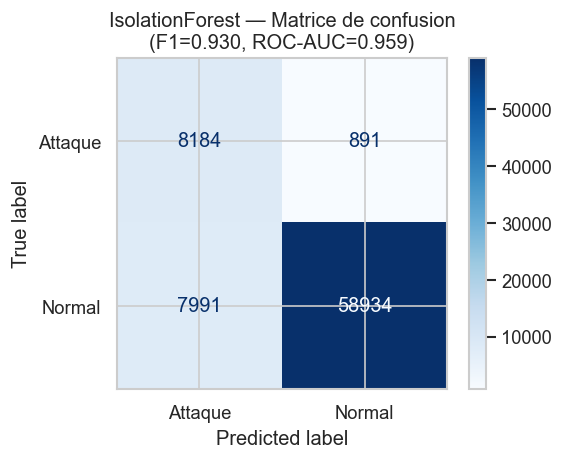
\includegraphics[width=0.6\textwidth]{figures/iso_forest_confusion_matrix.png}
  \caption{Matrice de confusion — IsolationForest}
  \label{fig:iso_cm}
\end{figure}

\section{Random Forest — Détection supervisée}

\subsection{Entraînement et optimisation}

\begin{lstlisting}[language=python, caption=Entraînement du Random Forest]
from sklearn.ensemble import RandomForestClassifier

rf = RandomForestClassifier(
    n_estimators=200,
    max_depth=None,
    min_samples_split=2,
    min_samples_leaf=1,
    class_weight='balanced',
    random_state=42,
    n_jobs=-1
)

rf.fit(X_train, y_train)
y_pred_rf = rf.predict(X_test)
\end{lstlisting}

\subsection{Résultats Random Forest}

\begin{table}[H]
\centering
\caption{Métriques Random Forest (détection binaire)}
\label{tab:rf_results}
\begin{tabular}{ll}
\toprule
\textbf{Métrique} & \textbf{Valeur} \\
\midrule
Précision & 0.994 \\
Rappel & 0.993 \\
F1-Score & \textbf{0.994} \\
ROC-AUC & \textbf{0.999} \\
\bottomrule
\end{tabular}
\end{table}

\begin{figure}[H]
  \centering
  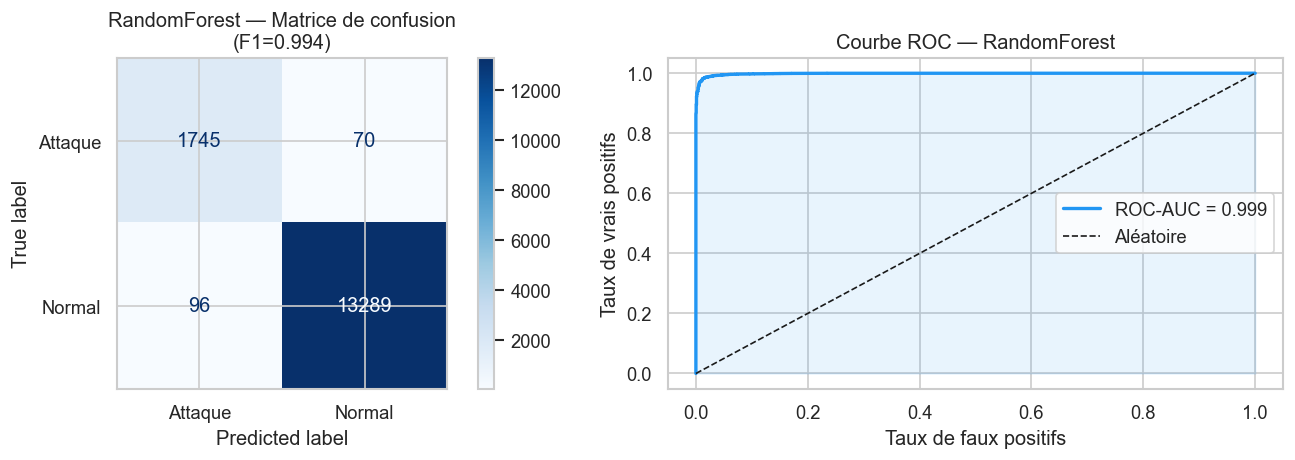
\includegraphics[width=\textwidth]{figures/rf_confusion_roc.png}
  \caption{Matrice de confusion et courbe ROC — Random Forest}
  \label{fig:rf_roc}
\end{figure}

\begin{figure}[H]
  \centering
  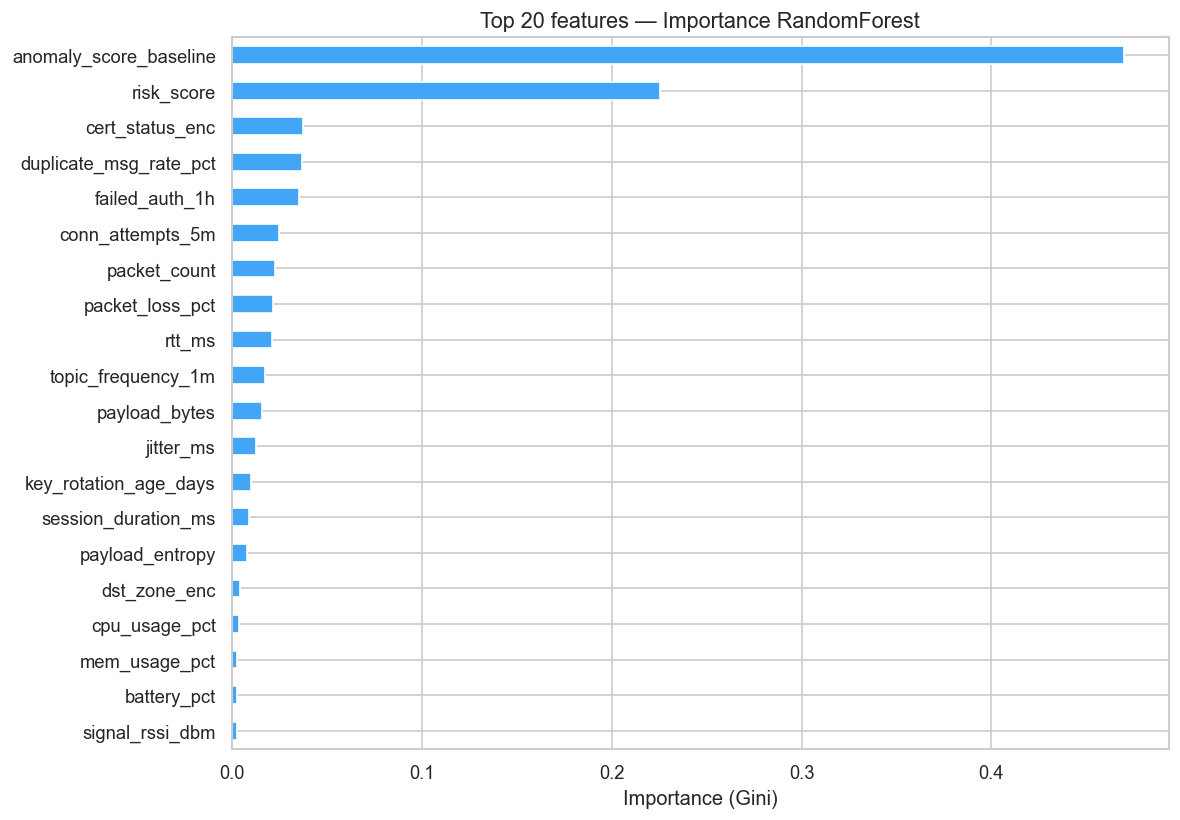
\includegraphics[width=0.8\textwidth]{figures/rf_feature_importance.png}
  \caption{Importance des features — Random Forest}
  \label{fig:rf_features}
\end{figure}

\subsection{Classification multi-classe}

Un deuxième modèle Random Forest a été entraîné pour la classification multi-classe (7 types d'attaques) :

\begin{figure}[H]
  \centering
  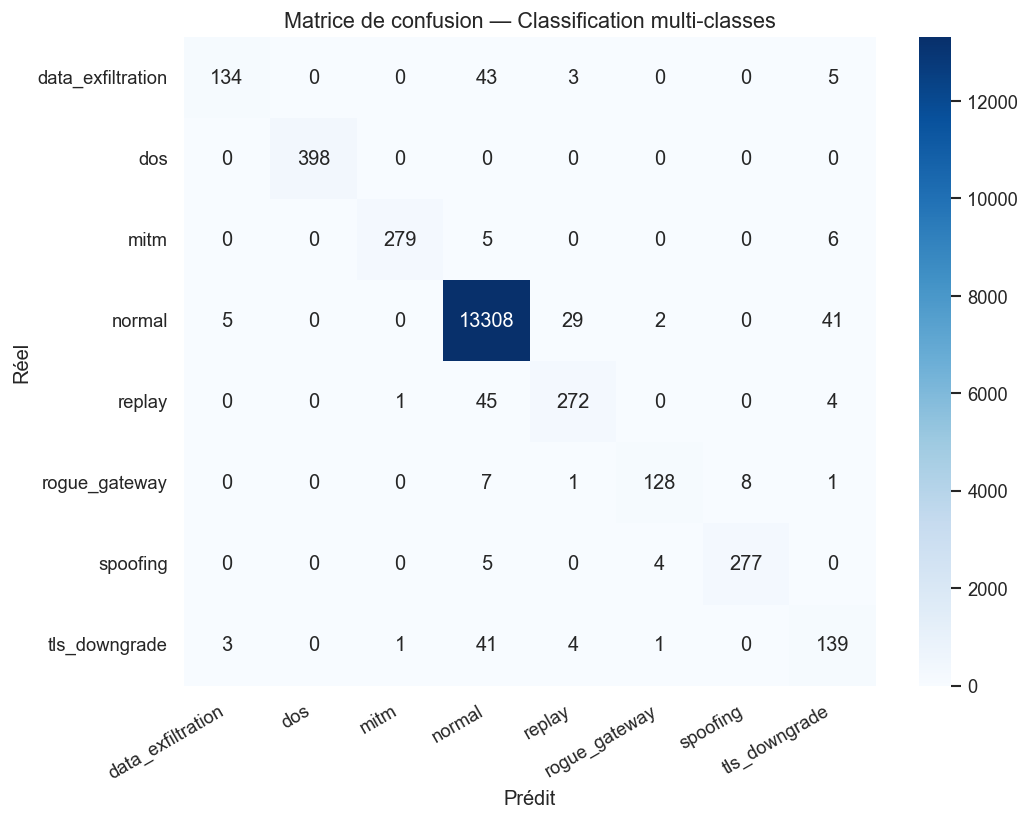
\includegraphics[width=0.8\textwidth]{figures/rf_multiclass_confusion.png}
  \caption{Matrice de confusion multi-classe — Random Forest}
  \label{fig:rf_multiclass}
\end{figure}

\section{Comparaison des modèles}

\begin{figure}[H]
  \centering
  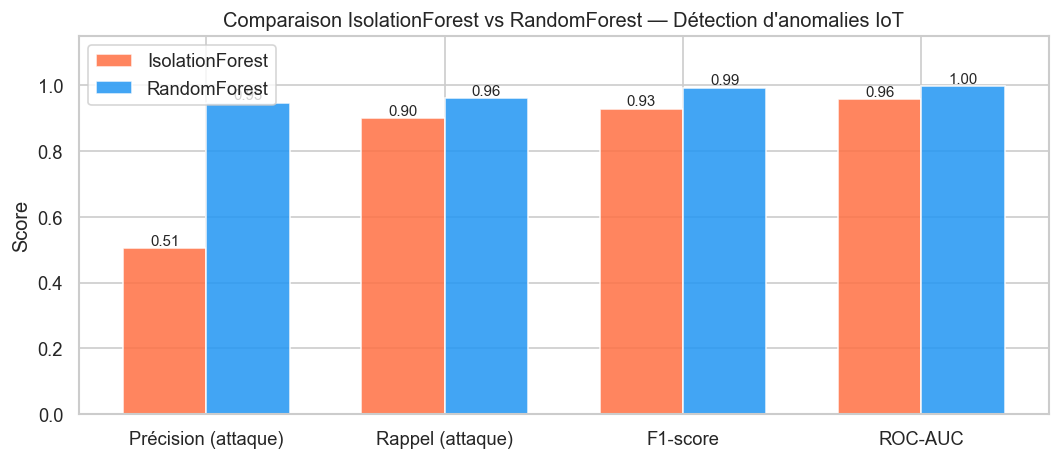
\includegraphics[width=0.8\textwidth]{figures/models_comparison.png}
  \caption{Comparaison IsolationForest vs Random Forest}
  \label{fig:models_comp}
\end{figure}

\begin{table}[H]
\centering
\caption{Comparaison finale des deux approches ML}
\label{tab:ml_comparison}
\begin{tabular}{llll}
\toprule
\textbf{Modèle} & \textbf{F1-Score} & \textbf{ROC-AUC} & \textbf{Type} \\
\midrule
IsolationForest & 0.930 & 0.959 & Non supervisé \\
Random Forest (binaire) & 0.994 & 0.999 & Supervisé \\
Random Forest (multi-classe) & 0.988 & 0.998 & Supervisé \\
\bottomrule
\end{tabular}
\end{table}

\begin{tcolorbox}[colback=green!5, colframe=green!50!black, title=Bilan ML]
Le Random Forest, en mode supervisé, atteint des performances quasi-parfaites (F1=0.994, ROC-AUC=0.999), exploitant les étiquettes pour apprendre les signatures de chaque attaque.

L'IsolationForest, sans étiquettes, obtient F1=0.930 — une performance remarquable pour un algorithme non supervisé, démontrant sa viabilité pour détecter des attaques inconnues dans des déploiements réels où les étiquettes ne sont pas disponibles.
\end{tcolorbox}
